When source identification is performed following initial detection of a
contamination incident, it is likely that the identified set of
possible injection locations is fairly large due to the limited
measurement information available at the early stages of detection.
As time progresses, more measurements become available to help
decrease the number of possible injection locations. It is possible to
obtain additional measurements in the form of grab samples from
optimally selected locations that can help in quickly narrowing down
the set of likely incident locations when source inversion
calculations are performed again. The \code{grabsample} subcommand can be used to
identify optimal grab sample locations 
that are likely to provide the most information in narrowing down the 
list of possible injection locations identified from
the \code{inversion} subcommand.

A flowchart representation of the \code{grabsample} subcommand is
shown in Figure \ref{fig:grabsample_flowchart}. The required input
for the \code{grabsample} subcommand includes a utility network model
specified with an EPANET 2.00.12 compatible input file (INP) and a list of
likely injection scenarios.
%A flowchart representation of the \code{grabsample} subcommand, used in conjunction with the 
%\code{inversion} subcommand, is shown in Figure \ref{fig:inversion_grabsample_flowchart}. 


\begin{figure}[h]
  \centering
  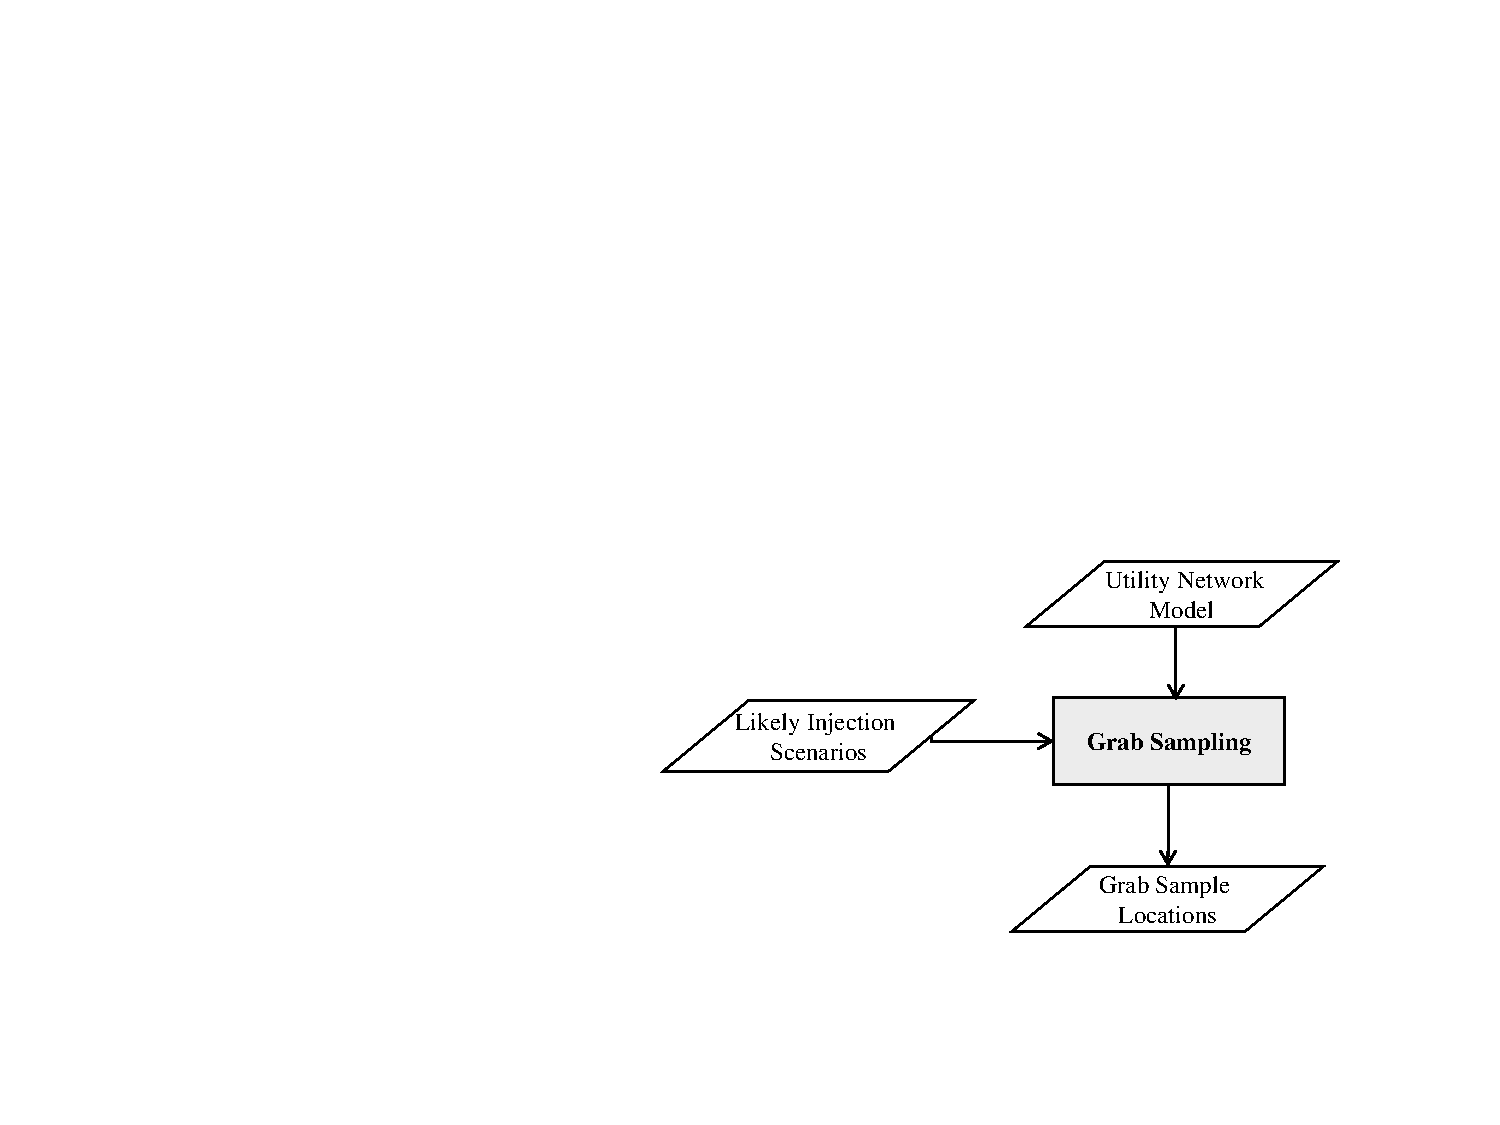
\includegraphics[scale=0.75]{graphics/grabsample_flowchart.pdf}
  \caption{Grab sample flowchart.}
  \label{fig:grabsample_flowchart}
\end{figure}

\section{Grab Sample Formulations}
The \code{grabsample} subcommand contains three different grab sampling formulations, 
the distinguishability formulation and two probability-based formulations.
The probability functions will likely be faster for larger problems (linear scaling), while the distinguishability formulation scales quadratically with the number of contamination scenarios. 
The following subsections provide brief descriptions of these formulations.

\subsection{Distinguishability Formulation}
\label{grabsample_formulation}
Considering two possible contamination incidents $i$ and $j$, if a
particular sample location is impacted by incident $i$, but not
impacted by incident $j$, then this sample location is able to
distinguish between the two incidents. The \code{grabsample} subcommand
can be used to identify grab sample locations that maximize the number
of pairwise distinguishable incidents in a list of possible
contamination incidents. The <output prefix>profile.tsg obtained
from the \code{inversion} subcommand contains a list of possible injection
locations. The data sets required by the optimization formulation
below are obtained by simulating each possible incident using the
EPANET 2.00.12 hydraulics model and either the EPANET 2.00.12 water quality model or the Merlion water quality model \citep{Mann1},
which can be selected using the merlion option in the scenario block of the configuration file.

The distinguishability problem formulation is:
\begin{align}
\textrm{maximize}\qquad &\sum_{(i,j) \in PE} d_{ij}\label{eqn.grabsample_obj}\\
\textrm{subject to} \qquad &\sum_{n \in D_{ij}}s_n \geq d_{ij} &&\forall \left( i,j \right) \in PE \label{eqn.grabsample_cons1} \\
&\sum_{n \in G}s_n \leq S_{\max} + \left|F\right|\label{eqn.grabsample_cons2} \\
&s_n \in \lbrace 0,1 \rbrace &&\forall \; n \in G \label{eqn.grabsample_cons3}\\
&s_n = 1 &&\forall \; n \in F \label{eqn.grabsample_cons5}\\
&0 \leq d_{ij} \leq 1 &&\forall \left( i,j \right) \in PE \label{eqn.grabsample_cons4}
\end{align}

where $G$ is the set of all grab sample locations, $F$ is the set of
fixed sensor locations and $PE$ is the pairwise set of all candidate
incidents (i.e., possible contamination incidents). The variable $D_{ij}$ is
the set of sample locations that distinguish incident $i$ from
incident $j$; $S_{max}$ is the maximum number of samples that can be
taken at the same time (i.e., number of sampling teams); $s_n$ is a
binary variable that is 1 if node $n$ is a good sample and is 0 otherwise; and
$d_{ij}$ is a continuous variable that will be 1 if incident $i$ is
distinguishable from incident $j$ and is 0 otherwise.

Equation \ref{eqn.grabsample_obj} represents the mixed-integer programming (MIP) objective, which
maximizes the number of pairwise distinguishable incidents.
Equation \ref{eqn.grabsample_cons1} requires that at least one or more
sample locations be selected for a distinguishable incident.
Equation \ref{eqn.grabsample_cons2} limits the number of selected
locations to be less than or equal to the number of sampling teams (specified by the user).
Equation \ref{eqn.grabsample_cons3} defines $s_n$ as a binary variable. 
Equation \ref{eqn.grabsample_cons5} ensures that the fixed sensor
locations are always sampled since measurements from these fixed sensors 
are always available, which avoids double counting distinguished incidents. This formulation is the default formulation solved in the \code{grabsample} subcommand.  

\subsection{Probability-based Formulations}
\label{probabilityFormulations}
From a source inversion perspective, the contamination incident that agrees with the largest number of measurements is the contamination incident with the higher probability of occurrence. Similarly, all contamination incidents that disagree with many of the measurements have a low probability of occurrence. Following this idea, two optimization formulations were implemented in the \code{grabsample} subcommand in order to determine optimal sampling locations that are intended to maximize the probability of identifying the true contamination incident (or minimizing the probability of incidents that did not occur).

\subsubsection{Maximization of expected number of scenarios that disagree with measurements}

Given a set of potential contamination incidents, a few scenarios will agree with all the measurements, while many more will disagree. For this reason, the formulations in this section aim to select locations that maximize the number of disagreements between incidents and measurements (quickly reduce the probabilities of the incidents that are not likely to be consistent with observations). The development of an MILP problem formulation that meets this goal is presented next.

\begin{align}
%& \underset{x, P_{s}^{\textrm{miss}}, P_{s}^{\textrm{match}}}{\textrm{max}} 
\textrm{maximize} \qquad&\;\; \sum_{s\in S}P_{s}^{\textrm{miss}} &  \label{eqn.p1_obj}\\
\textrm{subject to} \qquad &P_{s}^{\textrm{miss}} = 1-P_{s}^{\textrm{match}} & \;\forall \; s \in S \label{eqn.p1_c1}\\
&P_{s}^{\textrm{match}} = \exp(\tilde{P}_{s}) & \forall \; s \in S \label{eqn.p1_c2}\\
&\tilde{P}_{s} = \sum_{n\in N} x_n \ln(\alpha_{s,n}) & \forall \; s \in S \label{eqn.p1_c3}\\
&\sum_{n\in N} x_n \le S_{\textrm{max}} & \label{eqn.p1_c4}\\
&x_{n} \in \{0,1\} & \forall \; n \in N  \label{eqn.p1_c5}
\end{align}

Here $P_{s}^{\textrm{miss}}$ is the probability that incident $s$ disagrees with the outcome of the measurements at the selected locations. $P_s^{\textrm{match}}$ (complement of  $P_{s}^{\textrm{miss}}$) is given by the product of the probabilities $\alpha_{s,n}$ over all selected sampling locations,   

\begin{equation}
P_s^{\textrm{match}}= \prod_{n\in N} \alpha_{s,n}^{x_n}
\end{equation}

where $x_n$ is a binary variable that will be $1$ if location $n$ is selected for sampling, and is $0$ otherwise. In the formulation, this product is written in equations (\ref{eqn.p1_c2}) and (\ref{eqn.p1_c3}). The parameter $\alpha_{s,n}$ is the probability that incident $s$ disagrees with the outcome of a measurement taken at location $n$

\begin{equation}
\alpha_{s,n} = \left\{ \begin{array}{ll}
         \gamma_n & \mathrm{if }\ \delta_{s,n} = 1;\\
        1-\gamma_n & \mathrm{otherwise}.\end{array} \right. 
\label{alphasn}
\end{equation}

where $\delta_{s,n}$ is a binary parameter that is $1$ if incident $s$ contaminates node $n$, and $0$ otherwise. The values of $\delta_{s,n}$ are determined from the simulations pre-computed over the full potential incident set. The parameter $\gamma_n$ is the probability that node $n$ is contaminated and can be computed from the probability of the contamination incidents

\begin{equation}
\gamma_n = \sum_{s \in S} \delta_{s,n}\beta_s,
\label{nodeprob}
\end{equation}

Here $\beta_s$ is the current estimate of the probability of contamination incident $s$. Finally, $S_{\textrm{max}}$ is the maximum number of samples to be taken. The formulation as written is an MINLP because of Equation (\ref{eqn.p1_c2}). However, it is easily made linear. Note that the equality in Equation (\ref{eqn.p1_c2}) can be replaced with a lower bounding inequality. Since the objective function is maximizing $P_{s}^{\textrm{miss}}$ (and pushing down on $P_{s}^{\textrm{match}}$), this inequality will always be satisfied with equality at the solution. Note also that this new inequality is convex and can be replaced with a set of linear under-estimators.

This new MILP formulation, referred to as problem Probability1, is shown below, where $v_{i}$ are tangent
points selected for the linear under-estimators of the exponential term and $L$ is the set of indices corresponding to each of the linear under-estimators:

\begin{align}
%& \underset{x, P_{s}^{\textrm{miss}}, P_{s}^{\textrm{match}}}{\textrm{max}}
\textrm{maximize}\qquad & \;\; \sum_{s\in S}P_{s}^{\textrm{miss}} &  \label{eqn.p1_obj1}\\
\textrm{subject to}\qquad &P_{s}^{\textrm{miss}} = 1-P_{s}^{\textrm{match}} & \forall \; s \in S \label{eqn.p1_c11}\\
&P_{s}^{\textrm{match}} \geq \exp(v_i) + \exp(v_i) \left( \tilde{P}_{s} - v_i \right) & \forall \; i \in L, \; s \in S \label{eqn.p1_c21} \\
&\tilde{P}_{s} =  \sum_{n\in N} x_n \ln(\alpha_{s,n}) & \forall \; s \in S \label{eqn.p1_c31}\\
&\sum_{n\in N} x_n \le S_{\textrm{max}}  & \label{eqn.p1_c41}\\
&x_{n} \in \{0,1\} & \forall \; n \in N ,\label{eqn.p1_c51}
\end{align}

\subsubsection{Maximization of scenario with least number of measurement disagreements}

A third formulation is also presented that maximizes the worst-case number of mismatches (instead of the expected value). This formulation does not contain the exponential term and is already an MILP without the need for any linear under-estimators, which avoids numerical issues that can occur when too many numerically similar
under-estimators are added. This produces the max-min formulation shown below:
\begin{align*}
\textrm{maximize} \qquad \underset{s}{\textrm{minimize}} \qquad & P_{s}^{\textrm{miss}} &  \label{eqn.p2_bi_obj}\\
\textrm{subject to} \qquad &P_{s}^{\textrm{miss}} = 1-P_{s}^{\textrm{match}} & \forall \; s \in S \label{eqn.p2_bi_c1}\\
&P_{s}^{\textrm{match}} = \exp(\tilde{P}_{s}) & \forall \; s \in S \label{eqn.p2_bi_c2}\\
&\tilde{P}_{s} =  \sum_{n\in N} x_n \ln(\alpha_{s,n}) & \forall \; s \in S \label{eqn.p2_bi_c3}\\
&\sum_{n\in N} x_n \le S_{\textrm{max}}  & \label{eqn.p2_bi_c4}\\
&x_{n} \in \{0,1\} & \forall \; n \in N, \label{eqn.p2_bi_c5}\
\end{align*}
Recognizing that 
\[
\underset{s} \argmin \; P_{s}^{\textrm{miss}} = \underset{s}\argmin \;{-}P_{s}^{\textrm{match}} \label{eqn.p2_arg1}\\
\] 
and that 
\[
\underset{x} \argmin \; {-}x = \underset{x}\argmin \; {-}\exp(x), \label{eqn.p2_arg2}\\
\]
the prior bilevel optimization formulation is reformulated to a single level optimization formulation as, 

\begin{align}
\textrm{maximize} \qquad & \;\; q &  \\
\textrm{subject to} \qquad & \;\;q \leq -\tilde{P}_{s} & \label{eqn.p2_obj}\\
&\;\; \tilde{P}_{s} =  \sum_{n\in N} x_n \ln(\alpha_{s,n}) & \forall \; s \in S \label{eqn.p2_c1}\\
&\;\; \sum_{n\in N} x_n \le S_{\textrm{max}}  & \label{eqn.p2_c2}\\
&\;\; x_{n} \in \{0,1\} & \forall \; n \in N, \label{eqn.p2_c3}
\end{align}

This formulation is referred to as Probability2, where q is an auxiliary variable that
supports the max-min reformulation to a single level optimization problem.

\section{Grab Sample Solvers}
The \code{grabsample} subcommand requires standard MIP solvers to
identify optimal grab sample locations. The solvers recognized by
the \code{grabsample} subcommand are the same as those recognized
by \code{booster\_mip} subcommand (See
Section \ref{booster_mip_solver} for more details).
     
\section{\code{grabsample} Subcommand}

The \code{grabsample} subcommand is executed using the following
command line:
\begin{unknownListing}
wst grabsample <configfile>
\end{unknownListing}
where \code{configfile} is a WST configuration file in the YAML format. 

The \code{---help} option prints information about this subcommand:
\begin{unknownListing}
wst grabsample --help
\end{unknownListing}

\subsection{Configuration File}

The \code{grabsample} subcommand generates a template configuration
file using the following command line:

\begin{unknownListing}
wst grabsample --template <configfile>
\end{unknownListing}

The \code{grabsample} template configuration file is shown in
Figure \ref{fig:grabsample_template}. Brief descriptions of the
options are included in the template after the \# sign.

\begin{figure}[H]
  \unknownInputListing{examples/grabsample_config.yml}{}{1}{46}
  \caption{The \code{grabsample} configuration template file.}
  \label{fig:grabsample_template}
\end{figure}

The \code{grabsample} subcommand requires information about likely scenarios, which is set in the scenario block.
These scenarios must be defined using a TSG file or by specifying the scenario location, type, 
strength, start and stop times (see Section \ref{sec:scenarios} for more information on defining scenarios).
In general, the TSG file created by the \code{inversion} subcommand will be used to define likely scenarios.
Either the EPANET option or the Merlion option can be used as the water quality model, although, the Merlion
water quality model is recommended for larger networks. 


\subsection{Configuration Options}

Full descriptions of the WST configuration options used by
the \code{grabsample} subcommand are listed below.
\begin{description}[topsep=0pt,parsep=0.5em,itemsep=-0.4em]
  \item[{network}]\hfill
  \begin{description}[topsep=0pt,parsep=0.5em,itemsep=-0.4em]
    \item[{epanet file}]\hfill
\\ The name of the EPANET 2.00.12 input (INP) file that defines the water distribution
                network model.
                
                Required input.
  \end{description}
  \item[{scenario}]\hfill
  \begin{description}[topsep=0pt,parsep=0.5em,itemsep=-0.4em]
    \item[{location}]\hfill
\\A list that describes the injection locations for the contamination scenarios.
                The options are: (1) ALL, which denotes all nodes (excluding tanks and reservoirs)
                as contamination injection locations; (2) NZD, which denotes all nodes with
                non-zero demands as contamination injection locations; or (3) an EPANET node ID, 
                which identifies a node as the contamination injection location. This allows 
                for an easy specification of single or multiple contamination scenarios.
                
                Required input unless a TSG or TSI file is specified.
    \item[{type}]\hfill
\\The injection type for the contamination scenarios. The options are MASS, CONCEN, FLOWPACED or SETPOINT. 
                See the EPANET 2.00.12 user manual for additional information about source types \citep{EPANETusermanual}.
                
                Required input unless a TSG or TSI file is specified.
    \item[{strength}]\hfill
\\The amount of contaminant injected into the network for the contamination scenarios.  
                If the type option is MASS, then the units for the strength are in mg/min. 
                If the type option is CONCEN, FLOWPACED or SETPOINT, then units are in mg/L.
                
                Required input unless a TSG or TSI file is specified.
    \item[{species}]\hfill
\\The name of the contaminant species injected into the network. This is the name of a single species. 
                It is required when using EPANET-MSX, since multiple species might be simulated, but
                only one is injected into the network. For cases where multiple contaminants are injected,
                a TSI file must be used.
                
                Required input for EPANET-MSX unless a TSG or TSI file is specified.
    \item[{start time}]\hfill
\\The injection start time that defines when the contaminant injection begins. 
                The time is given in minutes and is measured from the start of the simulation. 
                For example, a value of 60 represents an injection that starts at hour 1 of the simulation.
                
                Required input unless a TSG or TSI file is specified.
    \item[{end time}]\hfill
\\The injection end time that defines when the contaminant injection stops.				
                The time is given in minutes and is measured from the start of the simulation.
                For example, a value of 120 represents an injection that ends at hour 2 of the simulation.
                
                Required input unless a TSG or TSI file is specified.
    \item[{tsg file}]\hfill
\\The name of the TSG scenario file that defines the ensemble of contamination
                scenarios to be simulated. Specifying a TSG file will
                override the location, type, strength, species, start and end times options specified in
                the WST configuration file. The TSG file format is documented in File Formats Section \ref{formats_tsgFile}.
                
                Optional input.
    \item[{tsi file}]\hfill
\\The name of the TSI scenario file that defines the ensemble of contamination
                scenarios to be simulated. Specifying a TSI file will
                override the TSG file, as well as the location, type, strength, species, start and end time options specified in
                the WST configuration file. The TSI file format is documented in File Formats Section \ref{formats_tsiFile}.
                
                Optional input.
    \item[{signals}]\hfill
\\Name of file or directory with information to generate 
                or load signals. If a file is provided, the list of INP-TSG tuples
                 will be simulated and the information stored in signals files. If
                a directory with the signals files is specified, the signal files will
                be read and loaded in memory. This input is only valid for the uq
                subcommand and the grabsample subcommand with probability based formulations.

                Optional input.
    \item[{msx file}]\hfill
\\The name of the EPANET-MSX multi-species file that defines the multi-species reactions to
                be simulated using EPANET-MSX.
                
                Required input for EPANET-MSX.
    \item[{msx species}]\hfill
\\The name of the MSX species whose concentration profile will be saved by the EPANET-MSX simulation
                and used for later calculations.
                
                Required input for EPANET-MSX.
    \item[{merlion}]\hfill
\\A flag to indicate if the Merlion water quality
                simulator should be used. The options are true or false. 
                If an MSX file is provided, EPANET-MSX will be used.
                
                Required input, default = false.
  \end{description}
  \item[{grabsample}]\hfill
  \begin{description}[topsep=0pt,parsep=0.5em,itemsep=-0.4em]
    \item[{model format}]\hfill
\\The modeling language used to build the formulation specified
                by the model format option. The options are AMPL and PYOMO. 
                AMPL is a third party package that must be installed by 
                the user if this option is specified. PYOMO is an open source 
                software package that is distributed with WST.
       
                Required input, default = PYOMO.
    \item[{sample criteria}]\hfill
\\ Determines which optimization model to solve. This option is 
                only checked when running the problem with signal files. By default
                the optimization is based on distinguishability of pair-wise scenarios.
       
                Optional input.
    \item[{sample time}]\hfill
\\The time at which the manual grab sample should be taken. 
                The algorithm determines the best possible manual grab sample location(s)
                based upon this time. Units: Minutes from the simulation start time in the
                EPANET 2.00.12 INP file. 

                Required input.
    \item[{threshold}]\hfill
\\This threshold determines whether or not an incident impacts a candidate
                sample location.

                Required input, default = 0.001.
    \item[{fixed sensors}]\hfill
\\A list that defines nodes that are already fixed continuous sensor locations.
                The options are: (1) ALL, which specifies all nodes as fixed sensor locations;
                (2) NZD, which specifies non-zero demand nodes as fixed sensor locations;
                (3) NONE, which specifies no nodes as fixed sensor locations;
                (4) a list of EPANET node IDs, which identifies specific nodes as fixed sensor locations; or
                (5) a filename, which references a space or comma separated file containing a list of 
                specific nodes as fixed sensor locations. 

                Optional input.
    \item[{nodes metric}]\hfill
\\ File containing a map of node to metric. The map is used for determining weighting factors
                in the objective of the distinguishability optimization formulation.
                Each line in the file has the node name separated by the corresponding metric.  

                Optional input.
    \item[{list scenario ids}]\hfill
\\ File containing list of scenarios to considered from the signals folder.
                Each line in the file has the signals ID and the contamination ID separated by a space.
				
                Optional input.
    \item[{feasible nodes}]\hfill
\\A list that defines nodes that can be considered as potential sampling locations 
                for the optimal sample location problem.
                The options are: (1) ALL, which specifies all nodes as feasible sampling locations;
                (2) NZD, which specifies all non-zero demand nodes as feasible sampling locations;
                (3) a list of EPANET node IDs, which identifies specific nodes as feasible sampling locations; or
                (4) a filename, which references a space or comma separated file containing a list of 
                specific nodes as feasible sampling locations. 

                Optional input.
    \item[{num samples}]\hfill
\\The maximum number of locations that can be sampled at one time. This is usually equal
                to the number of sampling teams that are available.

                Required input, default = 1.
    \item[{greedy selection}]\hfill
\\The option to select manual grab sample locations based upon a greedy search, which orders and selects the locations in order of the best solution.
                This does not require any optimization.

                Optional input, default = false.
    \item[{with weights}]\hfill
\\The option to add weights in the objective function of the distinguishability 
                optimization formulation.

                Optional input, default = false.
    \item[{filter scenarios}]\hfill
\\ This option enables filtering scenarios. Only those scenarios 
                that match at least one of the measurements are considered
                in the optimal sampling analysis.
				
				Optional input, default = false.
  \end{description}
  \item[{solver}]\hfill
  \begin{description}[topsep=0pt,parsep=0.5em,itemsep=-0.4em]
    \item[{type}]\hfill
\\The solver type. Each component of WST
				(e.g., sensor placement, flushing response, booster 
				placement) has different 
				solvers available. More specific details are provided in 
				the subcommand's chapter.
                
                Required input.
    \item[{options}]\hfill
\\A list of options associated with a specific solver type. More
            information on the options available for a specific solver
            is provided in the solver's documentation. The Getting
            Started Section \ref{dependencies} provides links to the
            different solvers.
            
            Optional input.
    \item[{threads}]\hfill
\\The maximum number of threads or function evaluations the solver is
                allowed to use.  This option is not available to all solvers or all analyses.
                
                Optional input.
    \item[{logfile}]\hfill
\\The name of a file to output the results of the solver.
                
                Optional input.
    \item[{verbose}]\hfill
\\The solver verbosity level.
                
                Optional input, default = 0 (lowest level).
    \item[{initial points}]\hfill
    \begin{description}[topsep=0pt,parsep=0.5em,itemsep=-0.4em]
      \item[{nodes}]\hfill
\\A list of node locations (EPANET IDs) to begin the optimization
        process. Currently, this option is only supported for the
        network solver used in the flushing and booster\_msx
        subcommands. This input causes an error for other subcommands.
        
        Optional input.
      \item[{pipes}]\hfill
\\A list of pipe locations (EPANET IDs) to begin the optimization
        process. Currently, this option is only supported for the
        network solver used in the flushing subcommand. This input causes an error for other subcommands.
        
        Optional input.
    \end{description}
  \end{description}
  \item[{configure}]\hfill
  \begin{description}[topsep=0pt,parsep=0.5em,itemsep=-0.4em]
    \item[{output prefix}]\hfill
\\The prefix used for all output files.
                
                Required input.
    \item[{output directory}]\hfill
      \\The output directory to store the results.
    \item[{debug}]\hfill
\\The debugging level (0 or 1) that indicates the amount of debugging 
                information printed to the screen, log file and output yml file. 
                
                Optional input, default = 0 (lowest level).
  \end{description}
\end{description}


\subsection{Subcommand Output}
The \code{grabsample} subcommand creates a YAML file called <output prefix>grabsample\_output.yml that contains
a list of node locations (EPANET node IDs) to 
take manual grab samples, the objective function value (based on the particular formulation selected), 
the run date and CPU time. 
The log file named <output prefix>grabsample\_output.log contains basic debugging information. 
A visualization YAML configuration file named <output prefix>grabsample\_output\_vis.yml is also created, and
following the execution of the \code{grabsample} subcommand, 
the \code{visualization} subcommand is automatically run using this YAML file.

\section{Grab Sample Examples}
Two examples for the \code{grabsample} subcommand are provided. The first example uses the distinguishability
formulation, while the second uses the probability-based formulation, Probability1.

\subsection{Example 1}
An EPANET 2.00.12 network model (INP format) and a file containing a list of
possible injection scenarios (e.g., a TSG file, which is generated by 
the \code{inversion} subcommand) are required to run the \code{grabsample} subcommand. The
configuration file for this example, grabsample\_ex1.yml, is shown in
Figure \ref{fig:sampling_ex1}. The EPANET Example Network 3 input file,
Net3.inp, is used for this example. 
The \code{grabsample} subcommand is typically used to identify sampling location 
after the results of the source identification calculation give a large list of
candidate injection nodes. The time line of using the \code{inversion} and \code{grabsample}
subcommand sequentially is provided in Figure \ref{fig:inversion_flowchart}.
The TSG file, Net3\_gs\_profile.tsg, which contains the possible contamination incidents, is created by the \code{inversion} subcommand using the measurement data created by the  \code{measuregen} executable (Executable Files Section \ref{measuregenExecutable}). For this example, the \code{measuregen} executable 
is used to simulate and obtain the measurements from a contaminant injection at node 251 at 24 hours.
The injection is detected at 30.5 hours by using a set of fixed sensor
locations defined in the Net3\_fixed\_sensors file.
The list of eight equally likely
contamination injection locations as listed in the TSG file, Net3\_gs\_profile.tsg, produced by the \code{inversion} subcommand is used as input to the 
\code{grabsample} subcommand along with the EPANET 2.00.12 network file. 
The sample time is set to 1890
minutes (31.5 hours), since it is assumed that it takes 60 minutes to
perform source identification and obtain the manual grab samples (including travel time). 
The maximum number of manual grab samples that can be taken is two.

\begin{figure}[H]
  \unknownInputListing{../../examples/grabsample_ex1.yml}{}{1}{32}
  \caption{The \code{grabsample} configuration file for example 1.}
  \label{fig:sampling_ex1}
\end{figure}

The example can be executed using the following command:
\begin{unknownListing}
wst grabsample grabsample_ex1.yml
\end{unknownListing}

The results are available in the {\outputprefix}grabsample\_output.yml, which
is shown in Figure \ref{fig:sampling_ex1_re}. The manual grab sample
locations identified are nodes 241 and 251. Twenty-three pairwise
incidents will be distinguished after taking the samples at these
locations. To reiterate the configuration parameters, the sampling
time is 1890 minutes and the maximum number of sampling locations is
two. The grab sample locations identified in Figure \ref{fig:sampling_ex1_re} 
might be one of several solutions that produce the same objective value. If 
multiple grab sample locations provide the same ability to distinguish the 
contamination source, the solver will randomly pick a solution. Thus, the solution 
identified in Figure \ref{fig:sampling_ex1_re} could be different for other users. 

\begin{figure}[H]
  \unknownInputListing{examples/sampling/grabsample_ex1_output.yml}{}{1}{13}
  \caption{The \code{grabsample} YAML output for example 1.}
  \label{fig:sampling_ex1_re}
\end{figure}

Next, as shown in Figure \ref{fig:inversion_flowchart}, the
measurements from these selected grab sample locations (actual or
simulated using \code{measuregen} executable) can be used to again
perform source identification. Please refer to
Section \ref{chap:inversionCase} for a complete case study of how to
use the \code{inversion} and \code{grabsample} subcommands in tandem.
 
\subsection{Example 2}

In the second example, the probability-based formulation, Probability1, is used to select the optimal sampling locations, since the probability-based formulations are particularly efficient when the number of contamination scenarios is considerably large. The configuration file for this example, grabsample\_ex2.yml, is shown in
Figure \ref{fig:sampling_ex2}. 

\begin{figure}[H]
  \unknownInputListing{../../examples/grabsample_ex2.yml}{}{1}{28}
  \caption{The \code{grabsample} configuration file for example 2.}
  \label{fig:sampling_ex2}
\end{figure}

The scenario information is provided with a list of pairs of INP-TSG files. This input allows the user to include different hydraulic and contamination in the set of potential scenarios. The list of potential scenarios used is shown in Figure \ref{fig:gs_scenarios}. Ten different INP files with variations in the demand patterns are specified in the list to account for uncertainty in the hydraulics of the system. For simplicity a single TSG file is specified to provide information about the contamination scenarios. However, each entry in the list of scenarios could have a different TSG file.

\begin{figure}[!ht]
  \unknownInputListing{../../examples/Net3/grabsample/list_scenarios.dat}{}{1}{10}
  \caption{List of scenarios example 2.}
  \label{fig:gs_scenarios}
\end{figure}

In addition, a list of the currently available measurements is provided in a measurement file with columns labeled as ``location, time and measurement value.'' The measurements are used to compute the probability of the scenarios following a Bayesian approach. When no measurements are provided, the probability distribution of the scenarios is assumed to be uniform. The measurement file in this example is shown in Figure \ref{fig:gs_measurements}

\begin{figure}[!ht]
  \unknownInputListing{../../examples/Net3/grabsample/MEAS.dat}{}{1}{3}
  \caption{List of measurements example 2.}
  \label{fig:gs_measurements}
\end{figure}

The example can be executed using the following command:
\begin{unknownListing}
wst grabsample grabsample_ex2.yml
\end{unknownListing}

The results are available in the {\outputprefix}grabsample\_output.yml, which
is shown in Figure \ref{fig:sampling_ex2_re}.

\begin{figure}[H]
  \unknownInputListing{examples/sampling/gs_ex2_output.yml}{}{1}{13}
  \caption{The \code{grabsample} YAML output for example 2.}
  \label{fig:sampling_ex2_re}
\end{figure}
